\section{Testbed Environment and Test Methodology}
\label{sec:testbed}

We used a Data Direct Networks (DDN) SFA10K as the storage backend for this
evaluation. SFA10K organizes disks into various RAID levels by two
active-active RAID controllers. In our testbed, exported RAID groups (LUNs) 
are driven by four server hosts (oss-[1-4]).  Each server host has
two InfiniBand (IB) QDR connections to SFA10K.  We used a single
dual-port Mellanox ConnectX IB QDR card per host.  By our calculation, this
setup is adequate to drive the SFA10K at its maximum theoretical throughput
(roughly 12 GB/s). 
%Server hosts and SFA10K connection diagram is illustrated in
%Figure~\ref{fig:ddn-sfa10k}.

\begin{comment}
\begin{figure}[htb]
\centering
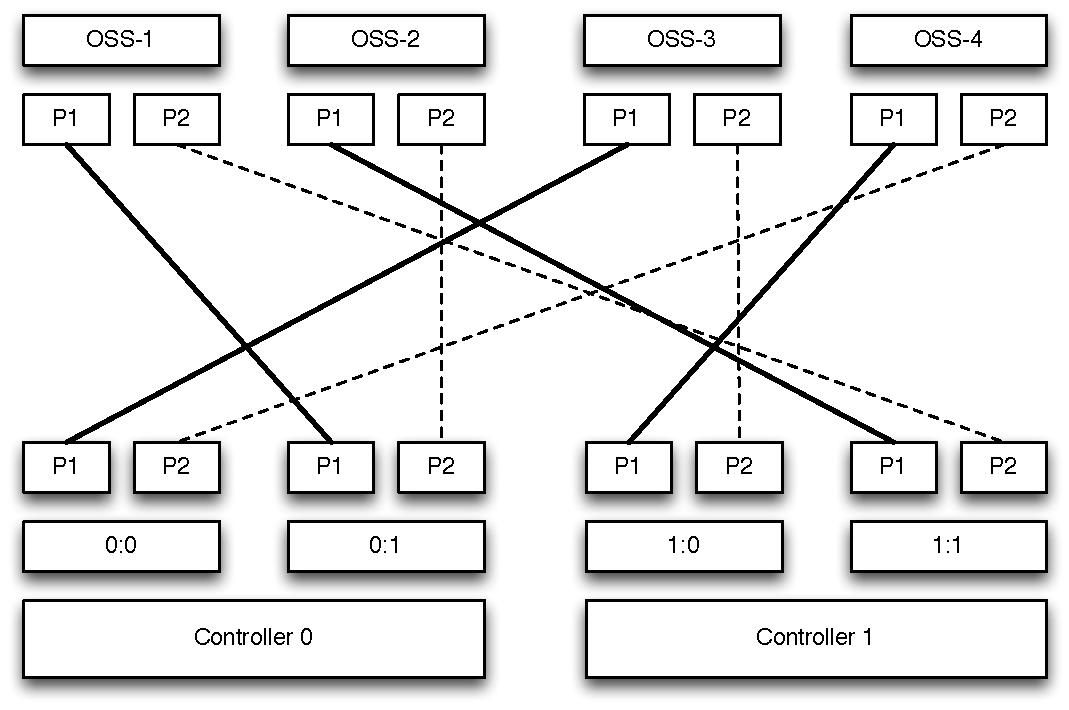
\includegraphics[width=3in]{figs/sfa10k}
\caption{DDN SFA10K hardware and host connection diagram}
\label{fig:ddn-sfa10k}
\end{figure}
\end{comment}

Our SFA10K system consists of 200 SAS drives and 280 SATA drives.
% hosted in a
%10-tray configuration. Each DDN SA4601 disk tray can host up to 60 disks and
%has two SAS links per controller (four in total). 
The SATA and SAS disks in our
testbed are distributed evenly over the SFA10K.
%ten SA4601 disk trays (20 SAS and 28 SATA
%disks per tray). 
Each SFA10K controller has two RAID processors and each
RAID processor hosts a dual-port IB QDR card. The disks are organized into RAID
groups by the RAID processors and then exported to connected
server hosts.
%over the IB connections. 
%Since each SFA10K controller is a
%stand-alone computer system running Linux, CPU and memory affinity while
%organizing disks into RAID groups and exporting them is crucial for obtaining
%top performance out of an SFA10K system.  

\begin{comment}
Our Ceph testbed employs a collection of nodes, including the server hosts
(oss-[1-4]). These nodes and their roles are summarized in
Table~\ref{tbl:ceph-test-nodes}. 
\end{comment}

%In the following discussion, we use ``servers'', ``osd servers'', ``server
%hosts'' interchangeably. We will emphasize with ``client'' prefix when we want
%to distinguish it from above.  
All hosts  (client and servers) were configured
with Redhat 6.3 and kernel version 3.5.1 initially, and later upgraded to 3.9,
Glibc 2.12 with syncfs support, locally patched.  We used the Ceph 0.48 and
0.55 release in the initial tests, upgraded to 0.64 and then to 0.67RC for a
final round of tests.


%%%%%%%%%%%%%%%%%%%%%%%%%%%%%% REMOVED
\begin{comment}
\begin{table}[!t]
\centering
\caption{Support nodes involved in Ceph testbed}
\label{tbl:ceph-test-nodes}
    \begin{tabular}{ll}
    \hline
    Node & Role \\
    \hline
    tick-mds1 & Ceph monitor node \\
    spoon46 & Ceph MDS node \\
    tick-oss[1-4] & Ceph OSD servers \\
    spoon28-31, spoon37-41 & Ceph client nodes \\
    \hline
    \end{tabular}
\end{table}
\end{comment}

%For a complete a list of hosts that are running ceph images, one can execute:

%\begin{Verbatim}
%$ grep "rhel6-ceph" /etc/gedi/MAC.info
%\end{Verbatim}


Our testing methodology is bottom to top. We start our evaluation from the
block-level to establish a baseline performance and work
our way up to the file system-level. We establish an expected
theoretical performance of a given hardware or software layer and then compare
that with the observed results of our experiments. Each added new layer to the
stack introduces new bottlenecks and re-defines the expected theoretical
performance of the overall system. 
%We will explain each component or layer and
%its expected performance before we present our observed results.

%Our tools for benchmarking and evaluating different layers also change as we
%go up in the stack.  For example, a tool perfect for assessing block-level
%performance over a single server host might be completely inadequate for
%observing parallel file system performance over multiple clients. As we
%present our evaluations, we will also introduce and explain our benchmark
%tools along the way.
